\documentclass[letterpaper,10pt,onecolumn]{article}
\usepackage[spanish]{babel}
\usepackage[latin1]{inputenc}
\usepackage{amsfonts}
\usepackage{amsthm}
\usepackage{amsmath}
\usepackage{mathrsfs}
\usepackage{empheq}
\usepackage{enumitem}
\usepackage[pdftex]{color,graphicx}
\usepackage{hyperref}
\usepackage{listings}
\usepackage{calligra}
\usepackage{algpseudocode} 
\DeclareMathAlphabet{\mathcalligra}{T1}{calligra}{m}{n}
\DeclareFontShape{T1}{calligra}{m}{n}{<->s*[2.2]callig15}{}
\newcommand{\scripty}[1]{\ensuremath{\mathcalligra{#1}}}
\lstloadlanguages{[5.2]Mathematica}
\setlength{\oddsidemargin}{0cm}
\setlength{\textwidth}{490pt}
\setlength{\textheight}{610pt}
\setlength{\topmargin}{-85pt}
\addtolength{\hoffset}{-0.3cm}
\addtolength{\textheight}{4cm}

\begin{document}
\thispagestyle{empty}
\begin{center}


\includegraphics[width=490pt]{figs/header.png}\\[0.5cm]

\textsc{\LARGE Parcial 2 - F\'isica I (FISI-1018) - 2016-10}\\[0.5cm]

\textsc{\Large{Profesor: Jaime Forero --- Fecha: Marzo 3, 2016}} \\[0.5cm]
\end{center}

Yo, \rule{10cm}{0.4pt}, con c\'odigo \rule{4cm}{0.4pt} de Uniandes,
acepto hacer este ex\'amen sin ayuda ni copia de fuentes no
permitidas (incluyendo libros, notas y cualquier dispositivo
electr\'onico excepto calculadoras digitales),  sabiendo que hacer lo
contrario va a ser considerado como fraude (una falta grave que se
sanciona hasta con suspenci\'on de la Universidad por dos semestres
como consta en el cap\'itulo X del reglamento general de estudiantes). 

\begin{enumerate}
\item \label{padrehijo}
Un adulto de masa $M$ sostiene a un ni\~no de masa $m$ con una cuerda
a trav\'es de una polea como se muestra en la Figura \ref{fig:padrehijo}. 
\begin{enumerate}
\item (10 puntos) Haga el diagrama de cuerpo libre sobre el adulto y
  el ni\~no.
\item  (10 puntos) Cu\'anto vale la normal (en Newton) que hace el
  piso sobre el adulto si $M=80$kg y $m=$10kg?
\end{enumerate}


\item \label{cable}
La barra que se muestra en la Figura \ref{fig:cable} (denotada por $AB$), esta
sostenida por el cable $BC$, el cual tiene un extremo fijo en el punto
$C$. Una persona aplica una fuerza de $1000$N a lo largo de BD con un
�ngulo de $20^{\circ}$ respecto a la vertical.  


\begin{enumerate}
\item  (10 puntos) Determine el valor de $\alpha$ para el cual la
  tensi�n es m�nima en el cable. 
\item (10 puntos) Encuentre la magnitud de la tensi�n para el �ngulo
  que encontr� en el inciso anterior.  
\end{enumerate}


\item 

Un autom�vil entra a una curva de radio $R$, la carretera tiene un
�ngulo de inclinaci�n $\theta$ y el coeficiente de fricci�n entre las
llantas y el asfalto es $\mu$, 
\begin{enumerate}
\item (10 puntos) Encuentre la m�xima velocidad que puede tener el carro para mantenerse en la carretera sin deslizarse de lado.
\item (10 puntos) Encuentre la m\'inima velocidad que puede tener el carro para mantenerse en la carretera sin deslizarse de lado.
\item (10 puntos) Qu\'e pasa en el caso $\mu=1$ y  $\theta=45^{\circ}$? 
\end{enumerate}



\item \label{bloques} Tenemos la configuraci\'on de bloques mostrada en la
  Figura \ref{fig:bloques}. Entre los bloques hay fricci\'on con
  coeficiente est\'atico $\mu$, pero entre los bloques y el piso no
  hay fricci\'on. Hay una fuerza $F$ externa que se aplica halando una
  cuerda atada al bloque $m_1$ a la derecha. 
\begin{enumerate}
\item(10 puntos) Haga un diagrama de cuerpo libre sobre cada uno de
  los cuatro cuerpos.
\item (10 puntos) Plantee la segunda ley Newton para cada uno de los
  cuatro cuerpos.
\item (10 puntos) Calcule la fuerza  {\bf m\'axima} $F$ que se puede
  hacer antes de que el bloque $m_1$ a la derecha empieze a deslizarse
  sobre el bloque $m_2$?
\end{enumerate}


\end{enumerate}

\begin{figure}[h]
\centering
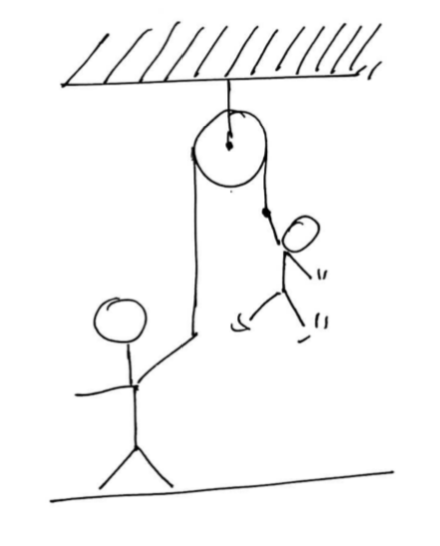
\includegraphics[width=0.30\textwidth]{padrehijo.png}\\
\caption{\label{fig:padrehijo}Figura para el ejercicio \ref{padrehijo}.}
\end{figure}

\begin{figure}[h]
\centering
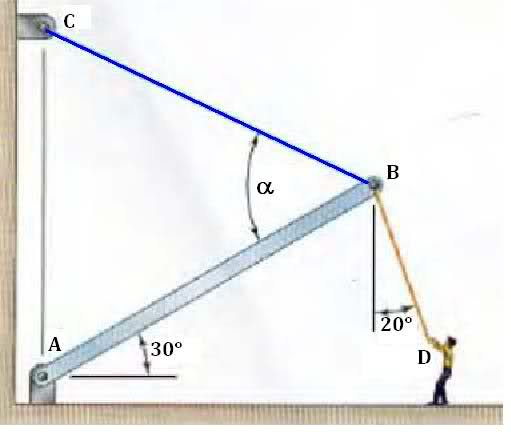
\includegraphics[width=0.40\textwidth]{complementariai1.jpg}\\
\caption{\label{fig:cable}Figura para el ejercicio \ref{cable}.}
\end{figure}


\begin{figure}[h]
\centering
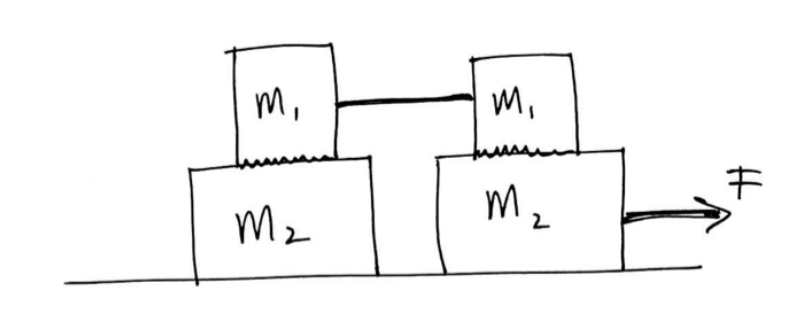
\includegraphics[width=0.40\textwidth]{bloques.png}\\
\caption{\label{fig:bloques}Figura para el ejercicio \ref{bloques}.}
\end{figure}

{\bf NOTA}: Todas las respuestas deben tener una justificaci\'on
f\'isica y matem\'atica adecuada. Tome $g=10$ m/s$^{2}$. 100 puntos
corresponden a una calificaci\'on de 5.0.
\end{document}
